

\section{Conversor Serial USB-RS485}
\label{conversor}


\begin{table}[ht!]

	\begin{tabular}{r l|l p{12cm} }
		
		\textcolor{gray}{Especificação} &&& 	{Conversor Serial USB-RS485}\\
		\textcolor{gray}{Data} &&& 				{30/07/2014}\\
        \textcolor{gray}{Beneficiado} &&&		{Prodigital Projetos Eletronicos} \\
        \textcolor{gray}{CNPJ} &&& 				{82.042.094/0001-26} \\
        \textcolor{gray}{Número Nota} &&& 		{5917} \\
		\textcolor{gray}{Quantidade} &&& 		{1} \\
		\textcolor{gray}{Valor} &&& 			{R\$399,00} \\
		\textcolor{gray}{Data Sheet} &&& 		{-} \\

		\textcolor{gray}{Função no projeto} &&& {O conversor USB-RS485 é utilizado
		durante testes de comunicação entre PC e sensor de pressão e também PC com
		microcontrolador.}
		\\
		\textcolor{gray}{Razão da Escolha} &&& {-}
		

	\end{tabular}
\end{table}

\newpage
\subsection{Foto do Material}
\begin{figure}[H]
 \centering
 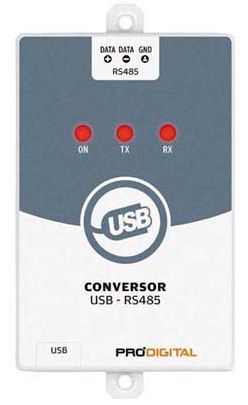
\includegraphics[width=0.5\columnwidth]{Conversor/foto}
 \caption{Conversor Serial USB-RS485}
\end{figure}

\subsection{Nota Fiscal}
\begin{figure}[H]
 \centering
 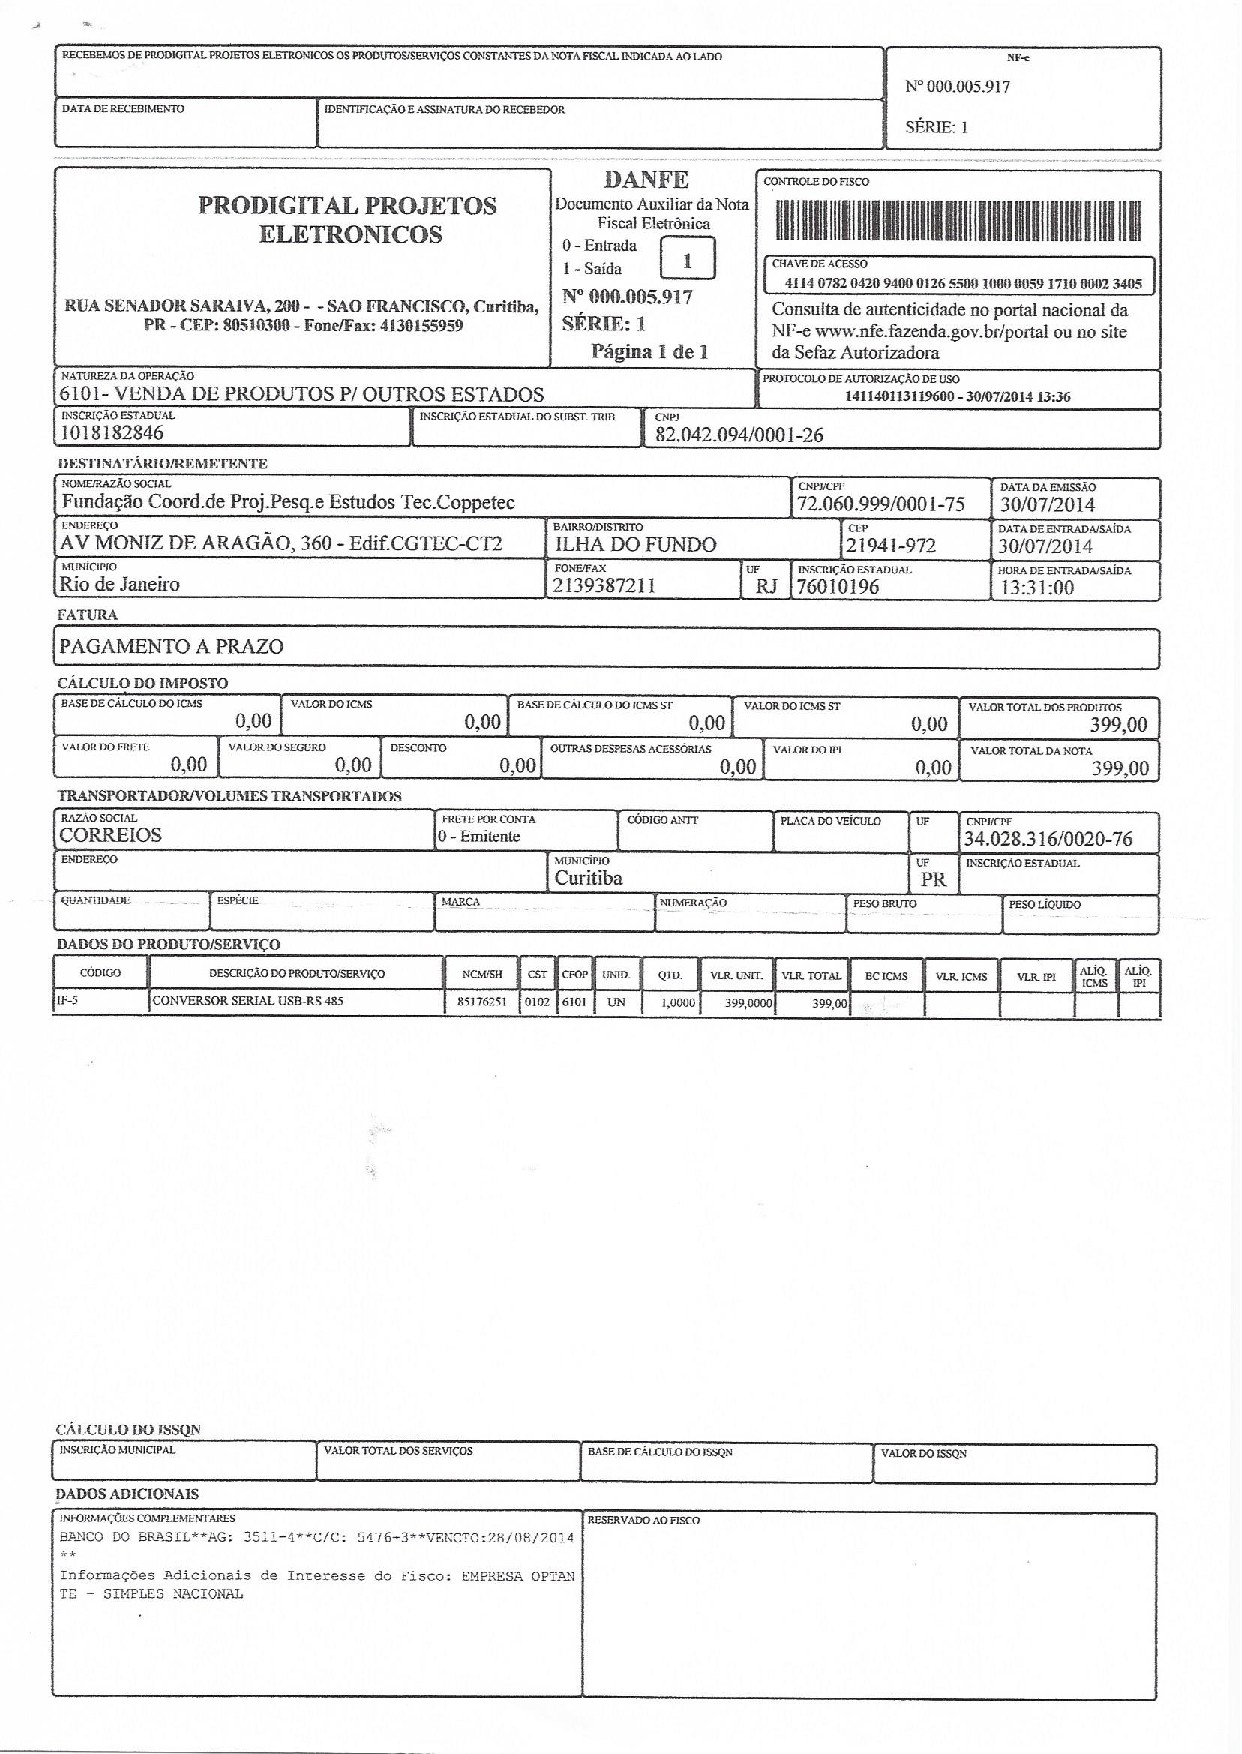
\includegraphics[width=0.9\columnwidth]{Conversor/nota_conversor.pdf}
 \caption{Conversor Serial USB-RS485}
 \end{figure}